%*******************************************************************************
% G?�wny dokument - tutaj definiowany jest g?�wny szablon ca?ej pracy
%*******************************************************************************

%===============================================================================
% plik stylu

%*******************************************************************************
% Definicje stylu dokumentu
%*******************************************************************************

%===============================================================================
% klasa dokumentu

\documentclass[12pt, a4paper, oneside, titlepage, final]{book}
%\documentclass[12pt,a4paper,onecolumn,oneside,11pt,wide,floatssmall]{book}


%===============================================================================
% Pakiety
%\usepackage[latin2]{inputenc}
\usepackage[cp1250]{inputenc}
%\usepackage[utf8]{inputenc}				% kodowanie �r�d�a
\usepackage[polish]{babel}				% polskie przenoszenie wyraz�w (hyph.)
\usepackage[OT4]{fontenc}					% font PL
\usepackage{url}								% polecenie \url
\usepackage{amsfonts}						% fonty matematyczne
\usepackage{graphicx}						% wstawianie grafiki
\usepackage{listings}						% wstawianie kodu
\usepackage{color}							% kolory
\usepackage{fancyhdr}						% paginy g�rne i dolne
\usepackage[plainpages=false]{hyperref}% dynamiczne linki
\usepackage{calc}								% operacje arytmetyczne w TeX'u
\usepackage{tabularx}						% rozci�gliwe tabele
\usepackage{array}							% standardowe tabele
\usepackage{hyperref}
\linespread{1.3}								% 1.3 do interlinii 1.5


% w�asne pakiety
\usepackage{pwtitle}

%===============================================================================
% Ustawienia dokumentu

\frenchspacing

% ustawienia wymiar�w
\oddsidemargin 20mm							% margines nieparzystych stron
\evensidemargin 20mm							% margines parzystych stron
\headheight 15pt								% wysoko�� paginy g�rnej
\topmargin 0mm									% margines g�rny

% styl paginacji
\pagestyle{fancy}
\renewcommand{\chaptermark}[1]{\markboth{#1}{}}
\renewcommand{\sectionmark}[1]{\markright{\thesection\ #1}{}}

% nag��wek 
\fancyhf{}
\fancyhead[L,RO]{\thepage}
\fancyhead[LO]{\small\nouppercase{\rightmark}}
%\fancyhead[R]{\small\nouppercase{\leftmark}}
\renewcommand{\headrulewidth}{0.1pt}
\renewcommand{\footrulewidth}{0pt}

% nag��wek w stylu plain 
\fancypagestyle{plain}
{
\fancyhf{}
\renewcommand{\headrulewidth}{0pt}
\renewcommand{\footrulewidth}{0pt}
}

% ta sekwencja tworzy czyste kartki na stronach po \cleardoublepage
\makeatletter
\def\cleardoublepage{\clearpage\if@twoside \ifodd\c@page\else
	\hbox{}
	\vspace*{\fill}
	\thispagestyle{empty}
	\newpage
	\if@twocolumn\hbox{}\newpage\fi\fi\fi}
\makeatother

%===============================================================================
% Zmienne �rodowiskowe i polecenia

% definicja
\newtheorem{definition}{Definicja}[chapter]

% twierdzenie
\newtheorem{theorem}{Twierdzenie}[chapter]

% obcoj�zyczne nazwy
\newcommand{\foreign}[1]{\emph{#1}}

% pozioma linia
\newcommand{\horline}{\noindent\rule{\textwidth}{0.4mm}}

% wstawianie obrazk�w {plik}{caption}{opis}
\newcommand{\fig}[3]
{
\begin{figure}[!htb]
\begin{center}
\includegraphics[width=\textwidth]{#1}
\caption[#2]{#2. #3}
\label{#1}
\end{center}
\end{figure}
}

%===============================================================================
% ustawienia pakietu hyperref

\hypersetup
{
%colorlinks=true,			% false: boxed links; true: colored links
%linkcolor=black,			% color of internal links
%citecolor=black,			% color of links to bibliography
%filecolor=black,			% color of file links
%urlcolor=black			% color of external links
}

%===============================================================================
% ustawienia pakietu listings

% kolor listingu
\definecolor{ListingBackground}{rgb}{0.97,0.97,0.97}

% ustawienia otoczenia
\lstset
{
language=C++,                   % choose the language of the code
basicstyle=\footnotesize,       % the size of the fonts
numbers=left,                   % where to put the line-numbers
numberstyle=\footnotesize,      % the size of the fonts for the line-numbers
stepnumber=1,                   % the step between two line-numbers.
numbersep=8pt,                  % how far the line-numbers are from the code
backgroundcolor=\color{white},  % choose the background color.
showspaces=false,               % show spaces adding particular underscores
showstringspaces=false,         % underline spaces within strings
showtabs=false,                 % show tabs within strings
frame=none,                     % adds a frame around the code
tabsize=3,                      % sets default tabsize to 2 spaces
captionpos=b,                   % sets the caption-position to bottom
breaklines=true,                % sets automatic line breaking
breakatwhitespace=false,        % sets if automatic breaks only at whitespace
escapeinside={(*@}{@*)},        % if you want to add a comment within your code
xleftmargin=1cm,
xrightmargin=0.5cm,
keywordstyle={\bf\footnotesize\color{blue}},
backgroundcolor={\color{ListingBackground}},
framexleftmargin=3pt,
framexbottommargin=3pt,
framextopmargin=3pt,
framexrightmargin=3pt,
frame=tb,
framerule=0.1pt
}

%===============================================================================
			% do??czanie plik�w stylu

\begin{document}

%===============================================================================
% Front

\frontmatter



\title{Indeksowanie obrazowych danych medycznych}
\author{Joanna Rogowska}
\promotor{prof. dr hab. in� Artur Przelaskowski}
\city{Warszawa}
\year{2013/2014\\}
\maketitle

\makestatement

\makebiography

\makesummary

{\tableofcontents}
			% definicja strony tytu?owej

%===============================================================================
% Rozdzia?y - dla porz?dku pliki dla ka?dego z rozdzia?�w znajduj� si? w oddzielnych katalogach

\mainmatter

%*******************************************************************************
% Rozdzia� pierwszy
%*******************************************************************************

\chapter{Wst�p}
\label{cha:wprowadzenie}

jak powinna dzia�a� wyszukiwarka:
- znajdowa� obrazy podobne anatomicznie niezale�nie od modalno�ci czy w pierwszej kolejno�ci pokazywa� podobne w danej modalno�ci?\\
Za pokazywanie danej modalono�ci przemawia fakt, �e ka�da modalno�� odpowiada za znalezienie obraz�w o podobnych patologiach (fizjologia) lub obrazowa� anatomicznie. Np. Je�eli zapytanie obrazem PET - typowo funkcjonalnym to nie oczekujemy znalezienia danego organu anatomicznego tylko obrazy podobne w obr�bie modalno�ci
%###############################################################################
\section{Cel pracy}
\label{sec:cel_pracy}
- skonstruowanie nowoczesnej wyszukiwarki obraz�w medycznych z intuicyjnym gui \\
(rozdzia� 2 ma za zadanie wykaza�, �e jest z tym spory problem)\\
- znalezienie obraz�w o podobnej modalno�ci \\
(rozdz. 2 ma wykaza�, �e zwykle nie s� rozr�niane modalno�ci obrazowania, a wyniki nie zawsze s� trafione)\\
nie jest potrzebna specjalistyczna wiedza diagnostyczna (radiologiczna?) do rozwi�zania tego zagadnienia\\

		% rozdzia? 1
%*******************************************************************************
% Rozdzia� drugi
%*******************************************************************************

\chapter{Cz�� 1 - studia literaturowe}
\label{cha:studia_literaturowe}

1987r - koncepcja system�w CBIR\\
1992r. - pierwszy system CBIR. T.Kato - elektroniczna galeria sztuki zawieraj�ca 205 obraz�w.

%###############################################################################\
\section{Przegl�d istniej�cych system�w CBIR}
\label{sec:Przegl�d istniej�cych system�w CBIR}

Podstaw� pracy powinno by� przejrzenie tego co istnieje. Co z tego, �e zabior� si� za system CBIR skoro nie wiem jakie jest zapotrzebowanie rynku.\\
Na pocz�tku najbardziej popularne wyszukiwarki dla przeci�tnych u�ytkownik�w - nie domkni�ty sektor danych obrazowych.\\
Potem analiza kilku system�w wyszukiwania obraz�w medycznych.\\
Na ko�cu podsumowanie i motywacja co jest w nich fajne a co nie.\\

\subsection{Google Image Search}
\label{sec:Google Image Search}

od 06.2011r. [z osi czasu na https://www.google.com/insidesearch/]\\
wej�cie: \\
- obraz lub url\\
wyj�cie: \\
- strona g��wna wyszukiwarki (google1.png) z wyszukiwaniami tekstowymi i wizualnymi\\

\begin{figure}
\centering
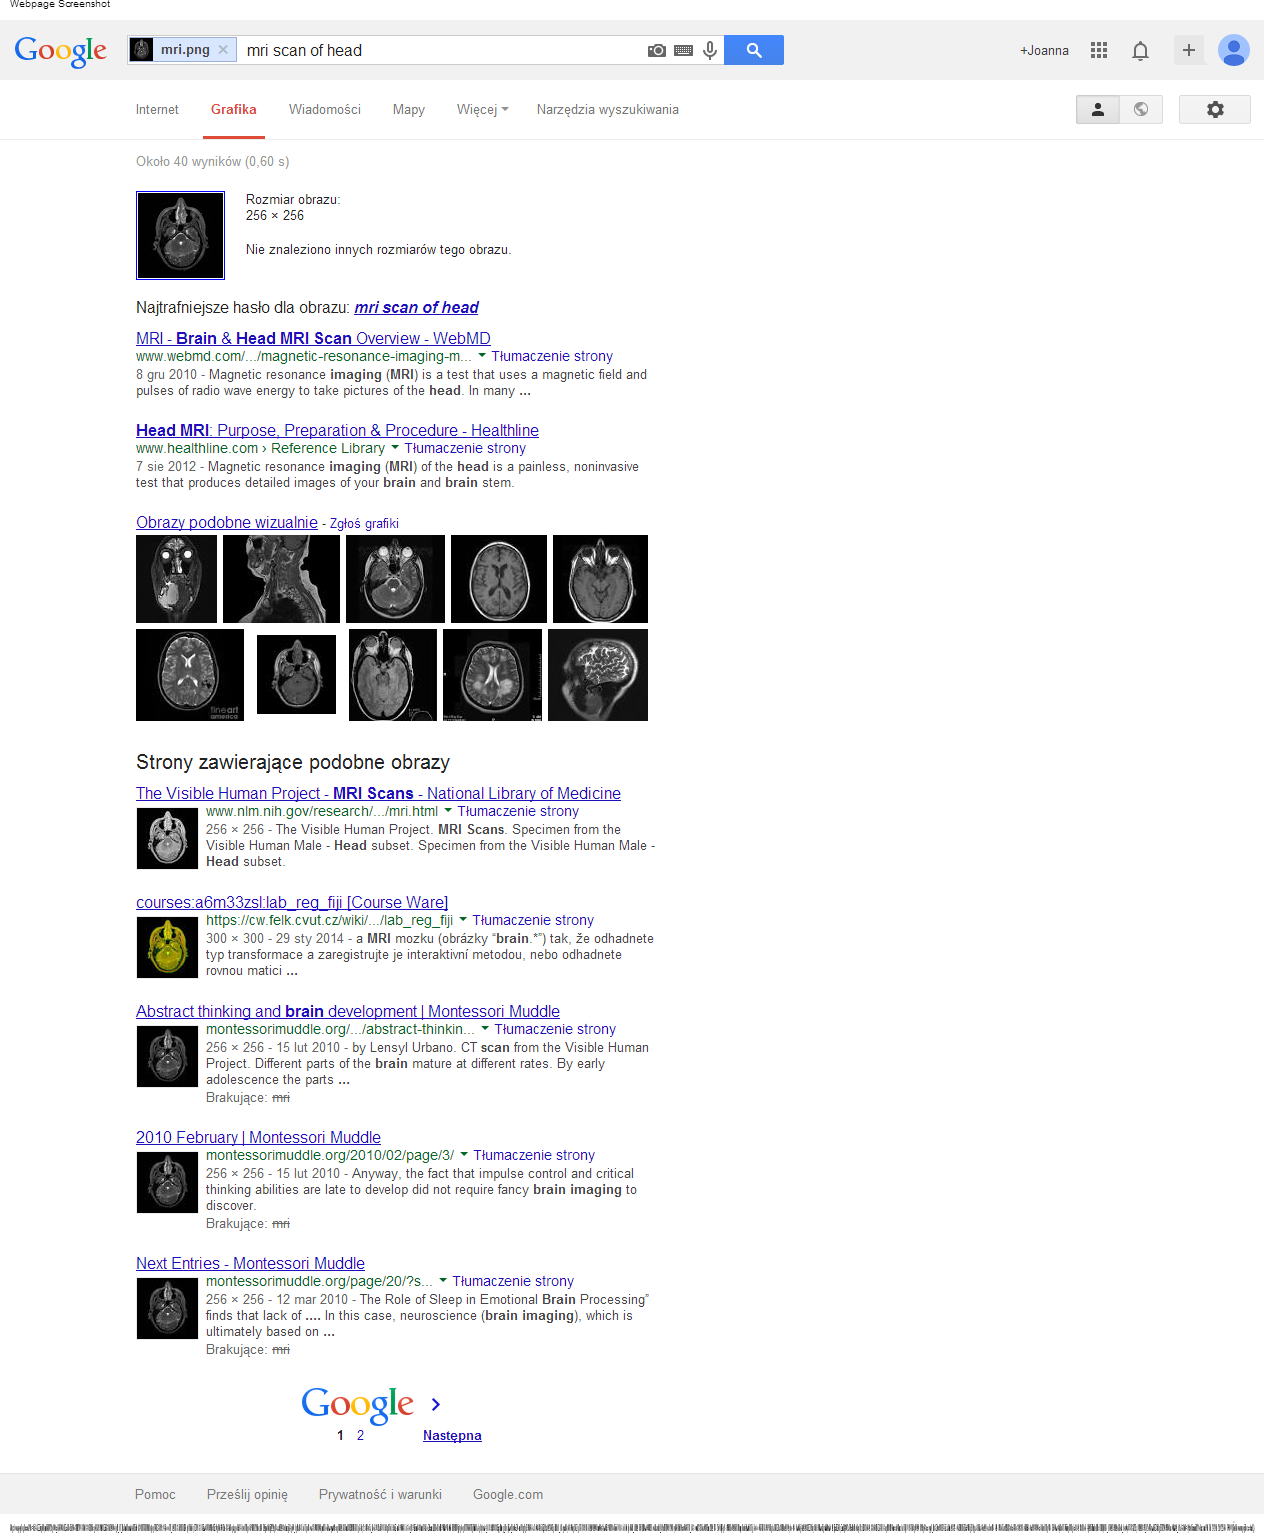
\includegraphics[scale=0.3]{Rozdzial02/Fig/google1.png}
\caption{\small Wynik wyszukiwania zapytania obrazem mri.png.}
\label{fig:google_image_search}
\end{figure}

wyniki wyszukiwania:\\
- konwertuje obraz na zapytanie tekstowe (rozr�nia mri od ct -> do dowiedzenia si� czy buduje to w oparciu o opisy obraz�w podobnych czy ma baz� wiedzy)\\
- wyniki (strony) dla wygenerowanego zapytania\\
- obrazy podobne wizualnie\\
- wyniki (strony) zawieraj�ce podobne obrazy\\


http://searchengineland.com/up-close-with-google-search-by-image-82313
radzi sobie ze znanymi obiektami (rozpoznaje muzea, obrazy itd), ma problem z mniej populanymi wyszukiwaniami jak, np. zdj�cia kwiat�w.

\subsection{Tineye}
\label{sec:Tineye}
Pierwszy webowy silnik do wyszukiwania obraz�w. 
wej�cie: \\
- obraz lub url\\
wyj�cie: \\
- znajdzie dok�adne dopasowania w tym te, kt�re zosta�y przyci�te, edytowane lub przeskalowane. Nie znajduje obraz�w podobnych.\\
wyniki wyszukiwania:\\
TinEye does not typically find similar images (i.e., a different image with the same subject matter); it finds exact matches including those that have been cropped, edited or resized.\\

Skoro nie znajduje podobnych to jakie jest zastosowanie?
There are many uses for TinEye, but here are a few:\\
Find out where an image came from, or get more information about it\\
Research or track the appearance of an image online\\
Find higher resolution versions of an image\\
Locate web pages that make use of an image you have created\\
Discover modified or edited versions of an image\\

to co fajne jest: jak si� kliknie w obrazek to por�wnuje znaleziony z wej�ciowym. Jaki� spos�b reprezentacji chc� u siebie zrobi� -> mo�e tak jak w �wierku? ko�o z przezroczysto�ci� ods�aniaj�ce tylko cz�� obrazu?

\subsection{IRMA}
\label{sec:irma}
obrazy radiologiczne.\\
na pocz�tku klasyfikacja do wybranych grup (drzewo TDBA). dla wej�cia buduje kod i szuka podobnych kod�w.\\


\subsection{Invisium?}
\label{sec:Invisium}
polskie zastosowanie komercyjne wspieraj�ce diagnostyk� medyczn�. Zawiera modu� wyszukiwania obraz�w podobnych. Skupia si� na znajdowaniu obraz�w u�ytecznych diagnostycznie

\subsection{wyszukiwarka obraz�w medycznych 3}
\label{sec:wyszukiwarka obraz�w medycznych 3}

%###############################################################################\
\section{Deskryptory numeryczne obraz�w medycznych}
\label{sec:deskryptory}

\subsection{CLEF Initiative}
\label{sec:CLEF Initative}

co roczny konkurs zwi�zany z przetwarzaniem obraz�w medycznych. Powstaj� opracowania ale nie powstaj� dzia�aj�ce programy w oparciu o uzyskane wyniki. Chc� je po��czy� wybrane z nich i zobaczy� czy posiadaj� praktyczne zastosowanie.\\
korzysta z baz danych IRMA

\subsection{MPEG-7}
\label{sec:MPEG-7}

CLD\\
EHD\\

\subsection{wagi skladowych deskryptorow}
\label{sec:wagi skladowych deskryptorow}

asdasd

%###############################################################################\
\section{Funkcje podobie�stwa}
\label{sec:Funkcje podobie�stwa}

asdasd

\subsection{cosinus pomi�dzy wektorami}
\label{sec:cosinus pomi�dzy wektorami}

sadas

\subsection{normy r�nych stopni}
\label{sec:normy r�nych stopni}

2-go stopnia (Euklidesowa)

niesko�czona


%###############################################################################\

%max 2-3 strony!!! standardowy temat. jest on celem przypomnienia i wprowadzenia poj�� potrzebnych w drugiej cz�ci pracy "praca w�asna"

\section{Sposoby analizy poprawno�ci zwr�conych wynik�w}
\label{sec:Sposoby analizy poprawno�ci zwr�conych wynik�w}

dsadad

\subsection{krzywe ROI?}
\label{sec:ROI}

asdasd

\subsection{Przywolanie}
\label{sec:Przywolanie}

asdasdasd

\subsection{Precyzja}
\label{sec:Precyzja}

asdasd		% rozdzia? 2
%*******************************************************************************
% Rozdzia� trzeci
%*******************************************************************************

\chapter{Cz�� 2 - badania w�asne}
\label{cha:badania_wlasne}

%###############################################################################
\section{Przyk�adowy podrozdzia�}
\label{sec:Przykladowy_podrozdzial_3}

Lorem ipsum dolor sit amet, consectetur adipiscing elit. Nam metus diam, fermentum dapibus volutpat id, posuere sit amet nisl. Sed nunc neque, tincidunt non mattis ut, eleifend a libero. Aenean feugiat gravida sem ac ullamcorper. Suspendisse potenti. Vestibulum a orci sit amet nulla pretium consectetur. Suspendisse euismod, est ut fringilla pretium, lacus metus lacinia magna, at tincidunt tortor nisi sit amet leo. Curabitur ultricies mauris quis mi vehicula feugiat. Nullam diam augue, auctor vitae imperdiet ut, blandit sit amet ipsum. Aliquam at velit et nibh suscipit hendrerit condimentum vel augue. Sed lacinia, augue quis egestas bibendum, erat metus dignissim lorem, id venenatis enim elit vitae augue. Duis est nisi, fermentum in cursus dignissim, molestie ac eros. Nunc egestas, tortor ut pretium convallis, metus leo vulputate nunc, ut bibendum nisi augue a enim. Phasellus molestie fringilla commodo. Donec arcu mi, cursus in gravida non, ullamcorper ut justo. Fusce gravida, odio in convallis interdum, quam turpis commodo enim, eu mattis nisl purus ac leo. Proin aliquet congue nisi, ac rutrum lorem dictum at. Nam ac iaculis tortor. Cras non justo erat, id adipiscing erat. Nunc molestie, purus et convallis vulputate, nibh nisl sagittis nibh, id ultrices urna risus rhoncus quam.


Quisque sapien nisi, euismod vel pulvinar et, commodo a neque. Fusce imperdiet volutpat quam, at vulputate velit tincidunt sed. Nulla tincidunt, ipsum porta luctus scelerisque, nulla enim egestas felis, at fringilla tortor ligula eu ipsum. Maecenas fringilla augue magna. Donec ut libero quis risus fringilla fermentum. Morbi lobortis consequat nisl. Etiam tellus metus, facilisis sit amet tempus at, molestie ac ligula. Praesent quis leo quam. Nam eget metus eu nibh dapibus molestie. Quisque volutpat interdum metus ut hendrerit. Suspendisse facilisis laoreet dapibus. Donec varius consequat aliquet. Phasellus at odio et sapien hendrerit tempor.

Nulla feugiat pretium convallis. Sed arcu eros, tincidunt at egestas sit amet, varius eu nunc. Vestibulum sollicitudin, tortor a feugiat mattis, tortor risus bibendum nulla, ac suscipit mi mi ut quam. Aenean id nibh magna, at dignissim est. Morbi augue magna, ultricies nec rutrum nec, feugiat sed dolor. Aliquam erat volutpat. Class aptent taciti sociosqu ad litora torquent per conubia nostra, per inceptos himenaeos. Lorem ipsum dolor sit amet, consectetur adipiscing elit. Cum sociis natoque penatibus et magnis dis parturient montes, nascetur ridiculus mus. Sed eu elementum purus. Cum sociis natoque penatibus et magnis dis parturient montes, nascetur ridiculus mus. Morbi luctus leo a elit sodales ac tempor risus condimentum. Aenean ut auctor ante.

Phasellus in purus arcu, at ultricies diam. Ut vestibulum sollicitudin est bibendum fermentum. Ut tempus faucibus arcu eu blandit. Proin adipiscing nisi eu massa egestas vestibulum. Integer sollicitudin ultrices massa ut aliquam. Maecenas enim justo, interdum lobortis pellentesque in, adipiscing nec tellus. Phasellus ac posuere nisi. Donec erat leo, consectetur in mattis sed, vehicula commodo ante. Pellentesque et mollis odio. Lorem ipsum dolor sit amet, consectetur adipiscing elit.

Integer quis nibh nec justo tristique bibendum. Proin posuere rhoncus erat, a bibendum magna posuere non. In tincidunt sollicitudin ipsum, at placerat libero ornare at. Mauris hendrerit. 
		% rozdzia? 3
%*******************************************************************************
% Rozdzia� czwarty
%*******************************************************************************

\chapter{Podsumowanie}
\label{cha:podsumowanie}

Lorem ipsum dolor sit amet, consectetur adipiscing elit. Nam metus diam, fermentum dapibus volutpat id, posuere sit amet nisl. Sed nunc neque, tincidunt non mattis ut, eleifend a libero. Aenean feugiat gravida sem ac ullamcorper. Suspendisse potenti. Vestibulum a orci sit amet nulla pretium consectetur. Suspendisse euismod, est ut fringilla pretium, lacus metus lacinia magna, at tincidunt tortor nisi sit amet leo. Curabitur ultricies mauris quis mi vehicula feugiat. Nullam diam augue, auctor vitae imperdiet ut, blandit sit amet ipsum. Aliquam at velit et nibh suscipit hendrerit condimentum vel augue. Sed lacinia, augue quis egestas bibendum, erat metus dignissim lorem, id venenatis enim elit vitae augue. Duis est nisi, fermentum in cursus dignissim, molestie ac eros. Nunc egestas, tortor ut pretium convallis, metus leo vulputate nunc, ut bibendum nisi augue a enim. Phasellus molestie fringilla commodo. Donec arcu mi, cursus in gravida non, ullamcorper ut justo. Fusce gravida, odio in convallis interdum, quam turpis commodo enim, eu mattis nisl purus ac leo. Proin aliquet congue nisi, ac rutrum lorem dictum at. Nam ac iaculis tortor. Cras non justo erat, id adipiscing erat. Nunc molestie, purus et convallis vulputate, nibh nisl sagittis nibh, id ultrices urna risus rhoncus quam.

Quisque sapien nisi, euismod vel pulvinar et, commodo a neque. Fusce imperdiet volutpat quam, at vulputate velit tincidunt sed. Nulla tincidunt, ipsum porta luctus scelerisque, nulla enim egestas felis, at fringilla tortor ligula eu ipsum. Maecenas fringilla augue magna. Donec ut libero quis risus fringilla fermentum. Morbi lobortis consequat nisl. Etiam tellus metus, facilisis sit amet tempus at, molestie ac ligula. Praesent quis leo quam. Nam eget metus eu nibh dapibus molestie. Quisque volutpat interdum metus ut hendrerit. Suspendisse facilisis laoreet dapibus. Donec varius consequat aliquet. Phasellus at odio et sapien hendrerit tempor.

Nulla feugiat pretium convallis. Sed arcu eros, tincidunt at egestas sit amet, varius eu nunc. Vestibulum sollicitudin, tortor a feugiat mattis, tortor risus bibendum nulla, ac suscipit mi mi ut quam. Aenean id nibh magna, at dignissim est. Morbi augue magna, ultricies nec rutrum nec, feugiat sed dolor. Aliquam erat volutpat. Class aptent taciti sociosqu ad litora torquent per conubia nostra, per inceptos himenaeos. Lorem ipsum dolor sit amet, consectetur adipiscing elit. Cum sociis natoque penatibus et magnis dis parturient montes, nascetur ridiculus mus. Sed eu elementum purus. Cum sociis natoque penatibus et magnis dis parturient montes, nascetur ridiculus mus. Morbi luctus leo a elit sodales ac tempor risus condimentum. Aenean ut auctor ante.
		% rozdzia? 4
% itd...

%===============================================================================
% Dodatki

\appendix

%*******************************************************************************
% Strona z dodatkami
%*******************************************************************************

\chapter{Dodatki}
\label{cha:dodatki}

%###############################################################################
\section{Przyk�adowa strona z dodatkami}
\label{sec:Przykladowy_dodatek}

Curabitur dui tellus, aliquam sit amet imperdiet eu, condimentum sit amet libero. Sed mollis turpis dolor, id consequat lorem. Maecenas sit amet urna eros. Praesent egestas egestas felis ut dignissim. Morbi posuere quam quam, eget lacinia libero. Morbi non urna tellus, vitae sagittis sem. Vestibulum ante ipsum primis in faucibus orci luctus et ultrices posuere cubilia Curae; Donec sed lectus velit, ut pretium ante. Etiam quis erat felis. Proin in nulla id libero commodo egestas ut a lacus. In elementum massa libero. Sed molestie enim sagittis lacus commodo commodo.

% przyk�ad u�ycia wzor�w
\begin{eqnarray}
 Z = \bigg((\mathrm {j} \omega L + R ) || \frac{1}{\mathrm {j} \omega C_1}\bigg) + \frac{1}{\mathrm {j} \omega C_2}
\end{eqnarray}
			% dodatki do pracy: wzory, obliczenia etc.

%===============================================================================
% Literatura

\backmatter

%*******************************************************************************
% Bibliografia - spis literatury wykorzystanej przy tworzeniu pracy
%*******************************************************************************

\begin{thebibliography}{99}
\addcontentsline{toc}{chapter}{Bibliografia}

\bibitem{1} Jan Stankowski, Wojciech Hilczer .: \emph{,,Wst�p do spektroskopii rezonans�w magnetycznych''}, Wydawnictwo Naukowe PWN, 2005.

\bibitem{2} Peter A.Rizzi .:  \emph{,,Microwave Engineering Passive Circuits''}, Prentice-Hall International Editions, 1988.


\end{thebibliography}
\clearpage

%===============================================================================
							% bibliografia

%===============================================================================
% Koniec

%*******************************************************************************
% Strony ko�cowe
%*******************************************************************************

%===============================================================================
% Spis rysunk�w - generowany automagicznie na podstawie deklaracji w tekscie

\listoffigures
\addcontentsline{toc}{chapter}{Spis rysunk�w}
\cleardoublepage

%===============================================================================
% O�wiadczenie

%\makestatement

%===============================================================================


\end{document}

%===============================================================================
